\section{第七周数值分析实验}
\subsection{Gram-Schmidt正交化}
\begin{ex}
	编程实现幂函数使用施密特正交化方法生成正交多项式
	
	施密特正交化:只要给定$[a,b]$上的权函数$\rho \left( x \right),$由$\{1,x,\cdots x^n,\cdots \}$利用逐个正交化立得正交多项式序列.
	$$
	\begin{aligned}
		& \varphi_0(x)=1, \\
		& \varphi_1(x)=x, \\
		& \varphi_2(x)=x^2-\frac{\left(x^2, \varphi_0\right)}{\left(\varphi_0, \varphi_0\right)} \varphi_0(x)-\frac{\left(x^2, \varphi_1\right)}{\left(\varphi_1, \varphi_1\right)} \varphi_1(x), \\
		& \varphi_n(x)=x^n-\sum_{j=0}^{n-1} \frac{\left(x^n, \varphi_j\right)}{\left(\varphi_j, \varphi_j\right)} \varphi_j(x), \quad n=3,4, \cdots .
	\end{aligned}
	$$
	或利用递推公式:
	$$
	\varphi_{n+1}(x)=\left(x-\alpha_n\right) \varphi_n(x)-\beta_n \varphi_{n-1}(x), n=0,1, \cdots
	$$
	其中
	$$
	\begin{aligned}
		& \varphi_0(x)=1, \varphi_{-1}(x)=0, \\
		& \alpha_n=\frac{\left(x \varphi_n(x), \varphi_n(x)\right)}{\left(\varphi_n(x), \varphi_n(x)\right)}, \beta_n=\frac{\left(\varphi_n(x), \varphi_n(x)\right)}{\left(\varphi_{n-1}(x), \varphi_{n-1}(x)\right)}, \\
		& \text { 这里 }\left(x \varphi_n(x), \varphi_n(x)\right)=\int_a^b x \varphi_n^2(x) \rho(x) d x .
	\end{aligned}
	$$
\end{ex}
\lstinputlisting[language=matlab]{day6/Schmidt1.m}
\subsection{Schmidt正交化-Legendre多项式}
\lstinputlisting[language=mathematica]{day6/schmidtlegendre.wl}
\qa (Mathematica)
\begin{figure}[H]
	\centering
	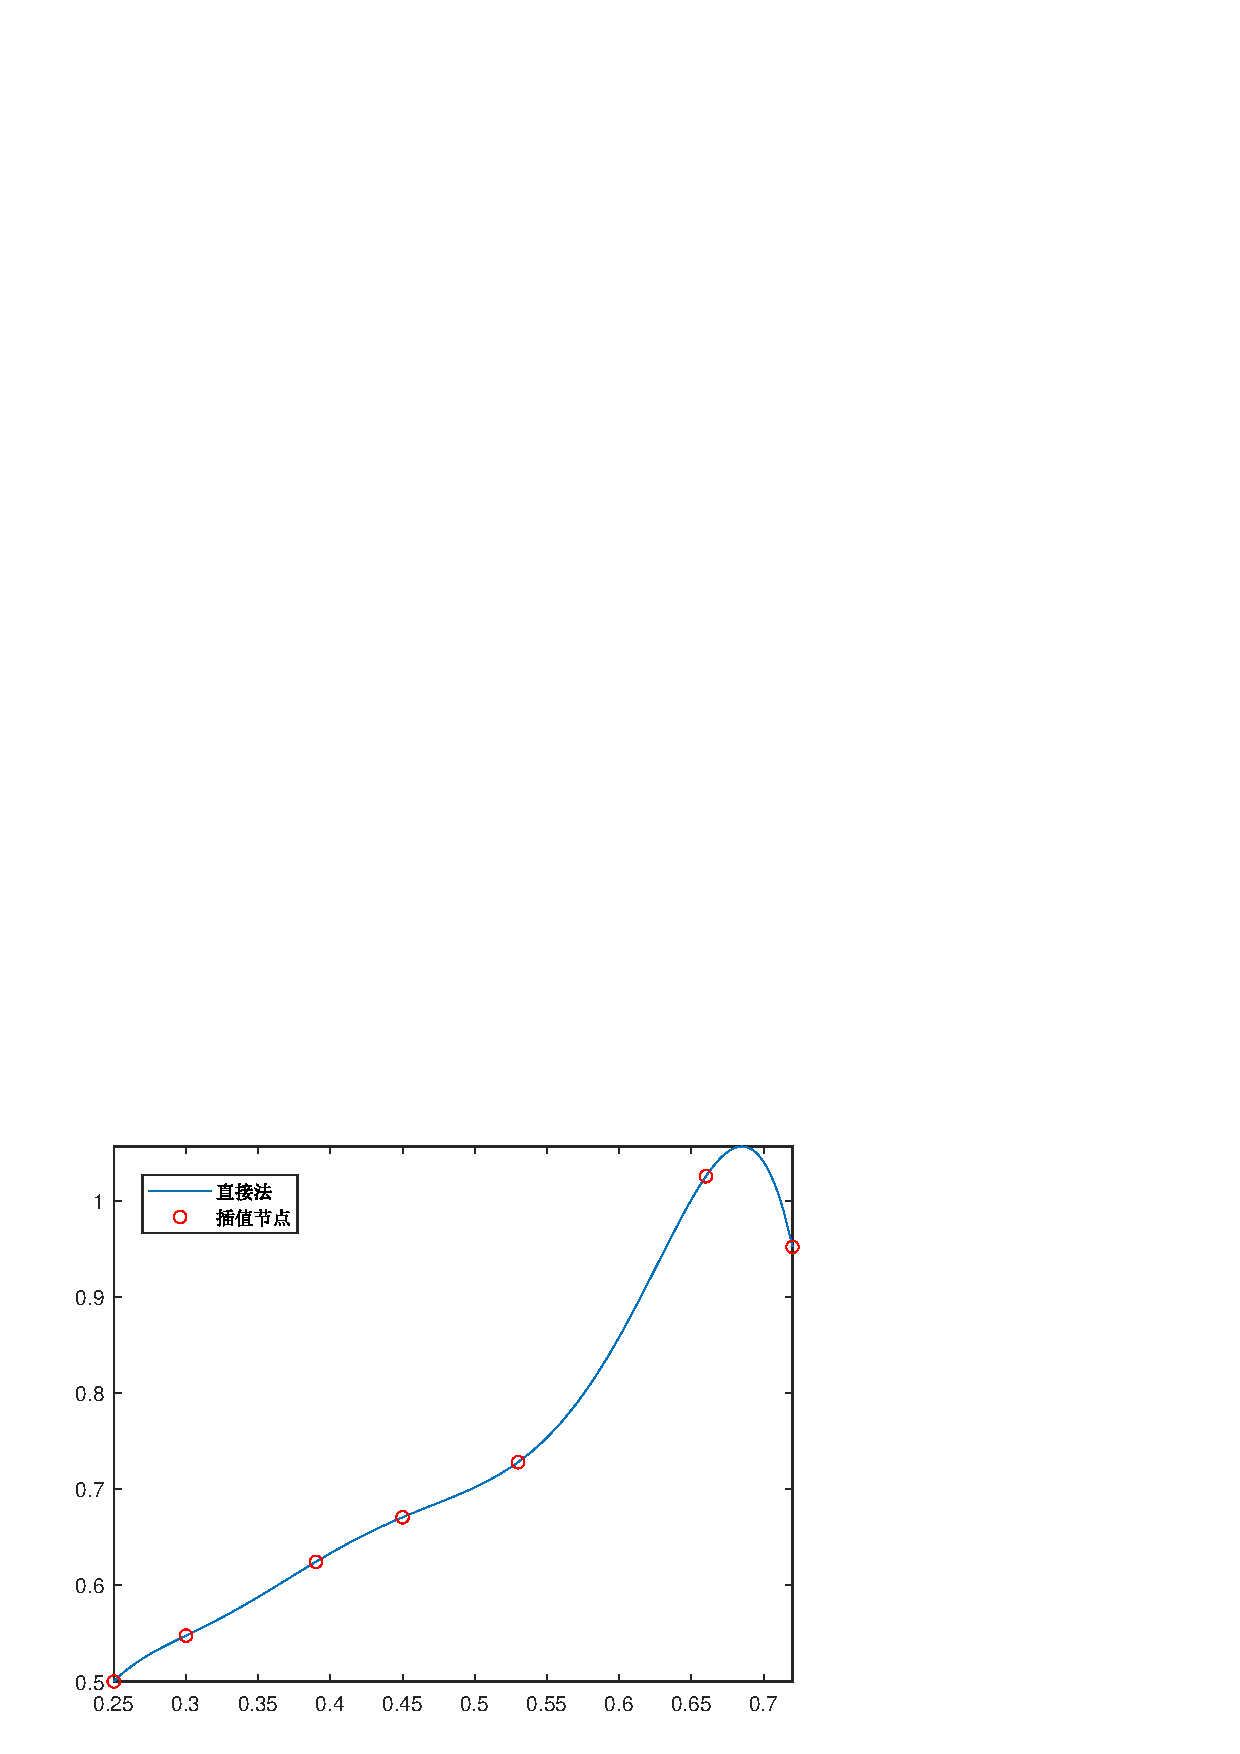
\includegraphics[width = 1\linewidth]{day6/fig1.png}
	\caption{Legendre}
\end{figure}
\subsection{Schmidt正交化-Chebyshev多项式}
\lstinputlisting[language=mathematica]{day6/schmidtchebyshev.wl}
\qa (Mathematica)
\begin{figure}[H]
	\centering
	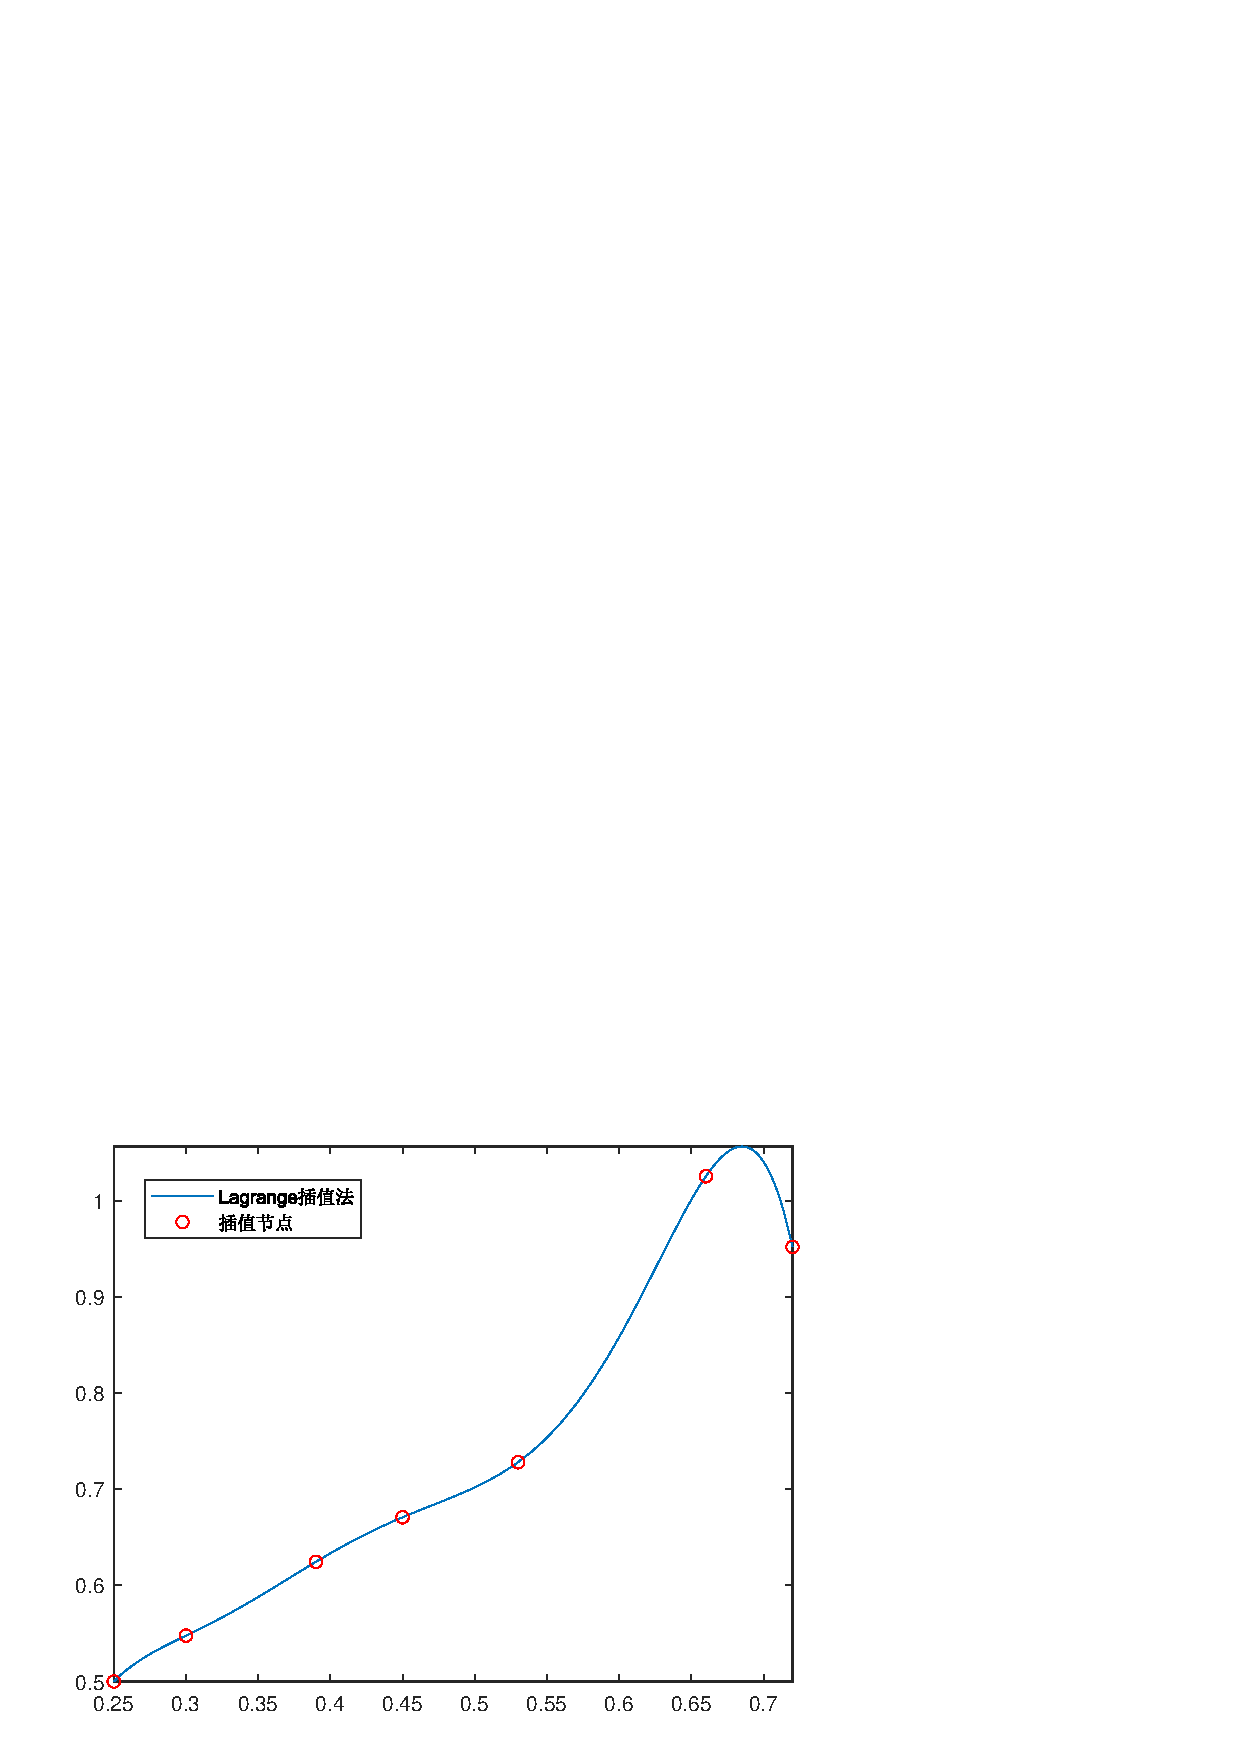
\includegraphics[width = 1\linewidth]{day6/fig2.png}
	\caption{Chebyshev}
\end{figure}
\subsection{递推法-Legendre多项式}
\lstinputlisting[language=matlab]{day6/legendremap.m}
